\documentclass[a4paper]{article}

\usepackage[utf8]{inputenc}
\usepackage{graphicx}
\usepackage{float}
\usepackage[caption = false]{subfig}
\usepackage{amsmath}
\usepackage{indentfirst}
\usepackage{hyperref}
\usepackage[margin=2.8cm]{geometry}

\title{Workflow documentation}
\author{Gustave Li}
\date{Last updated: July 2021}

\begin{document}

\maketitle

\section{Introduction}
The Carotenoid-Porphyrin-\(\text{C}_{60}\) (\(\text{CPC}_{60}\)) triad molecule consists of a porphyrin covalently linked with a carotenoid and a \(\text{C}_{60}\) molecule (Figure~\ref{fig:CPC60}). Carotenoid is the excited-state electron donor and the \(\text{C}_{60}\) serves as the electron acceptor, while porphyrin acts as a bridge to separate the two parts and transfer electrons. The molecule is a mimicry of the natural photosynthetic center which utilize photons to initiate a complex series of electronic transitions to achieve a high-energy charge separated state. It absorbs UV visible light and produces a charge separated state (\(\text{CT}_{2}\)) where an electron is transferred from C to \(\text{C}_{60}\), producing a large dipole moment of 150 D. Due to its outstanding performance in photoinduced charge transfer, it has a great potential in organic solar cells.

\begin{figure}[H]
    \centering
    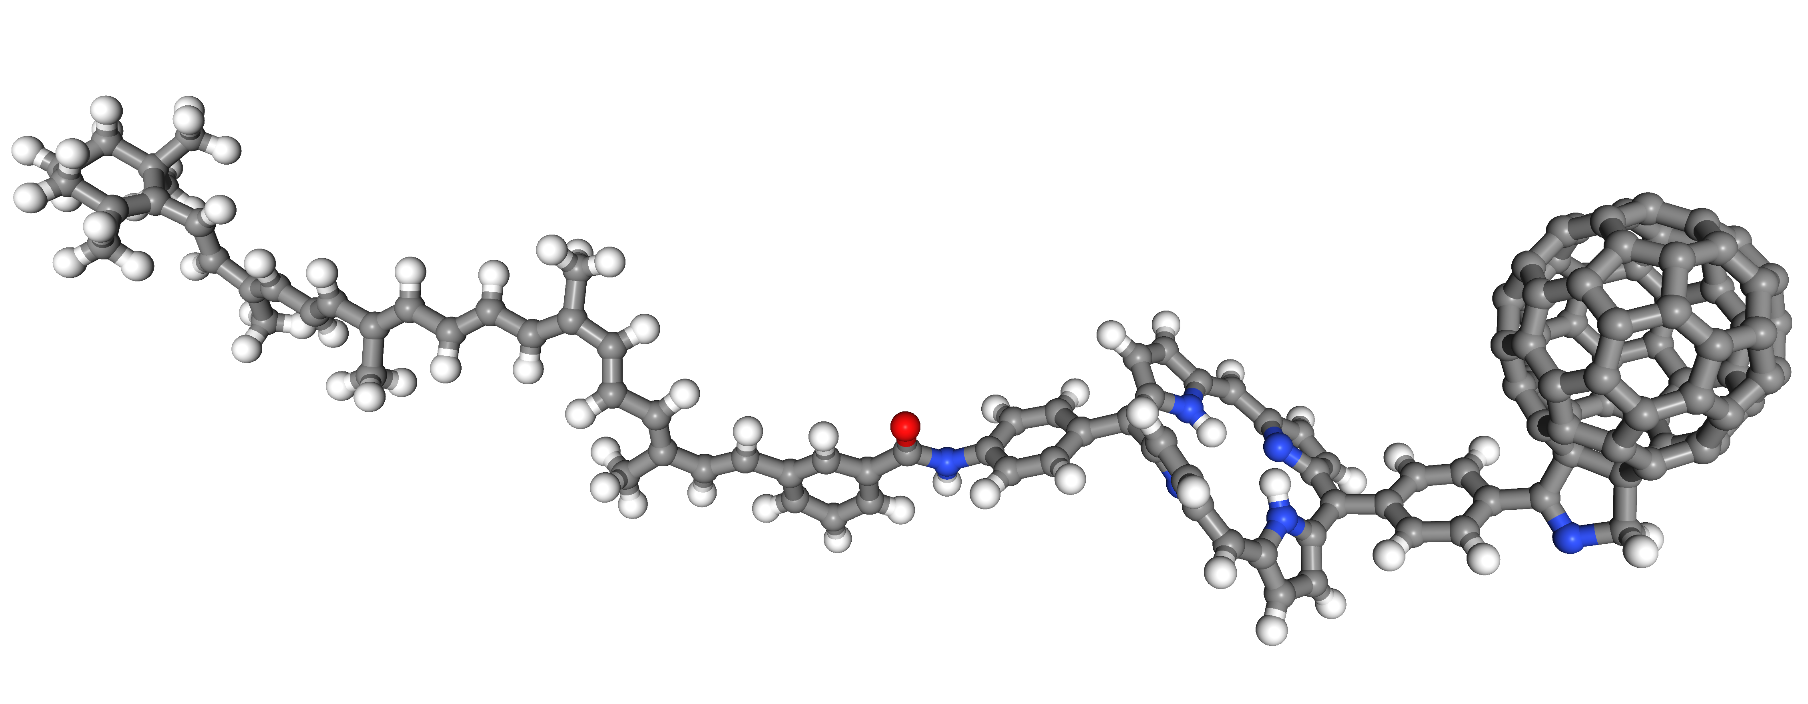
\includegraphics[width=0.75\linewidth]{projects/Gustave_Li/Docs/Triad.png}
    \caption{The \(\text{CPC}_{60}\) molecule}
    \label{fig:CPC60}
\end{figure}

However, Manna et al. reported that the triad spatial conformation strongly affects the process of charge separation and concluded that the linear conformations have better charge separation effeciency over the bent conformations \cite{MannaArun}. Olguin et al. further investigated the effect of structural changes on \(\text{CPC}_{60}\) charge transfer states, they summarized several factors influencing charge transfer, including donor-acceptor distance, distances and torsions between the three components \cite{OlguinMarco}. In summary, the charge transfer process in \(\text{CPC}_{60}\) is very conformation-dependent,  the molecular structure has a rather dramatic effect on the the charge transfer performance. Thus, finding the optimal structure for charge transfer is critical.

Thanks to the development of computer sciences, tens of thousands of possible \(\text{CPC}_{60}\) molecules can be generated based on molecular dynamics. Considering the heavy computing load of calculation and the complexity of the \(\text{CPC}_{60}\) molecule, it is unrealistic to calculate the charge transfer rate for all the molecules. Researchers are currently working on different directions to address this issue. Brian and co-worker proposed novel formulations for calculating charge transfer rate, which reduced a maximum of 80\% of computational cost \cite{BrianDomi}. In this project, we aim to make use of machine learning to cluster the many molecules into different groups. By taking the cluster center as representation conformations, we expect the computational cost to decrease for a great amount while maintaining as much structural information as possible.
\pagebreak

\section{Triad molecule visualization}
The triad molecule trajectory was loaded with the python \texttt{mdtraj} module, and the \texttt{nglview} module was applied for visualization. The ball-and-stick representation of the 100,000 triad molecules in the dataset was obtained, which is similar to that in Figure~\ref{fig:CPC60}. 

All the 100,000 molecules follow the same C-P-\(\text{C}_{60}\) sequence, but the overall conformation varies from bent to linear. Torsion around carotenoid-porphyrin and porphyrin-\(\text{C}_{60}\) also exists.

\section{Descriptors}
The goal of this project is to cluster the thousands of triad molecules, so different descriptors are needed to represent the features of molecules for machine learning algorithms to work. 

\subsection{Key atoms}
The key atoms chosen for descriptors are \(\text{C}_{33}\), \(\text{C}_{21}\), \(\text{C}_{61}\), \(\text{C}_{65}\), \(\text{C}_{66}\), \(\text{C}_{69}\), \(\text{C}_{89}\), \(\text{C}_{95}\), \(\text{C}_{96}\), \(\text{C}_{128}\) and \(\text{N}_{6}\) (Figure \ref{fig:key_atoms})

\begin{figure}[H]
    \centering
    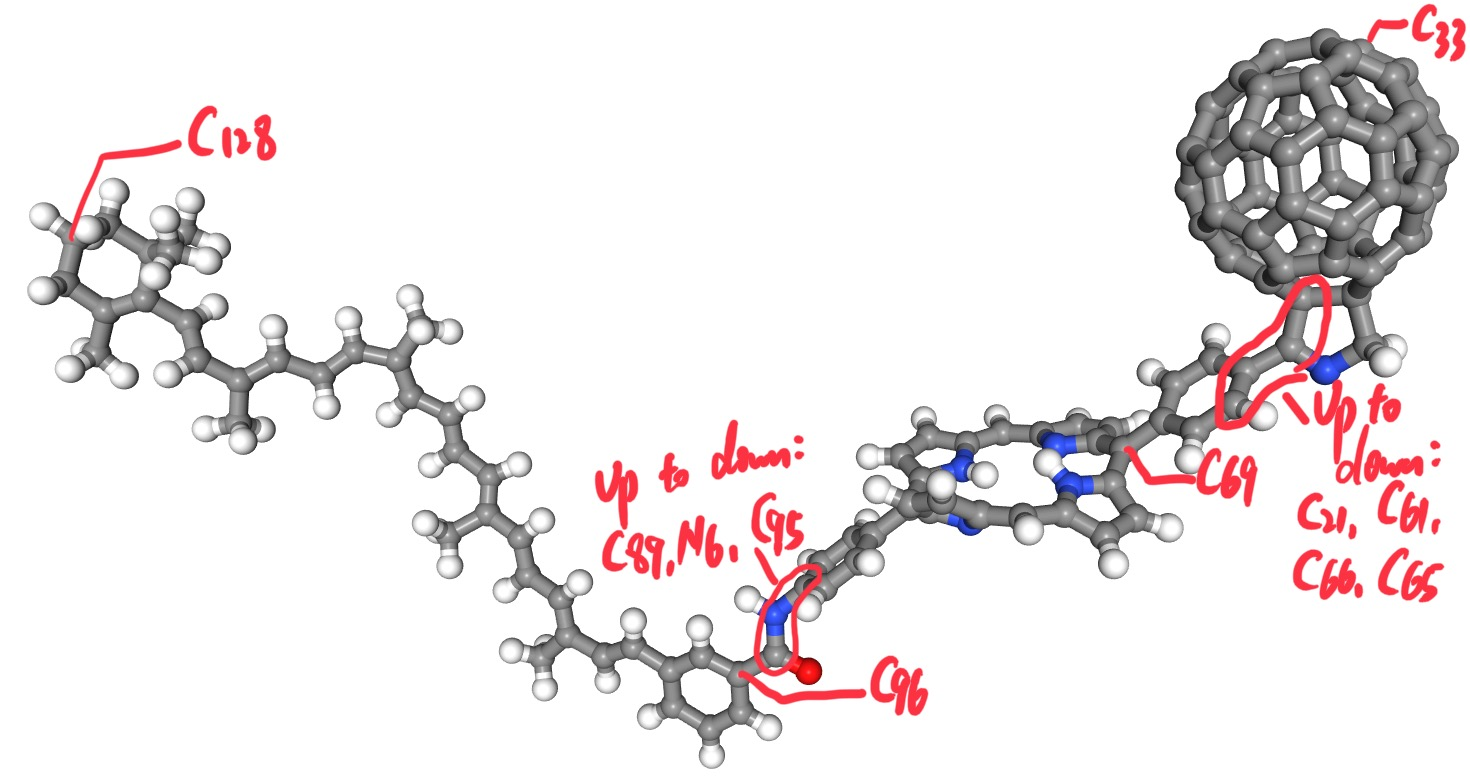
\includegraphics[width=0.75\linewidth]{projects/Gustave_Li/Docs/Key-atoms.jpg}
    \caption{Key atoms for descriptors}
    \label{fig:key_atoms}
\end{figure}

\subsection{Geometric descriptors}
\begin{table}[ht]
    \centering
    \caption{Definitions of geometric descriptors}
    \begin{tabular}{c|c}
    \hline \hline
       \textbf{Name}  & \textbf{Description} \\
       \hline \hline
       EuclidianDist\_1 & The euclidian distance between \(\text{C}_{33}\) \& \(\text{C}_{128}\) \\
       Angle\_1 & The angle between atoms \(\text{C}_{33}\)-\(\text{C}_{96}\)-\(\text{C}_{128}\) \\
       Angle\_2 & The angle between atoms \(\text{C}_{33}\)-\(\text{C}_{69}\)-\(\text{C}_{96}\) \\
       Angle\_3 & The angle between atoms \(\text{C}_{69}\)-\(\text{C}_{96}\)-\(\text{C}_{128}\) \\
       Dihedral\_1 & The absolute valute of dihedral between atoms \(\text{C}_{21}\)-\(\text{C}_{61}\)-\(\text{C}_{66}\)-\(\text{C}_{65}\) \\
       Dihedral\_2 & The absolute valute of dihedral between atoms \(\text{C}_{89}\)-\(\text{N}_{6}\)-\(\text{C}_{95}\)-\(\text{C}_{96}\) \\
       RMSD\_Linear & RMSD for the conformation to the Linear triad \\
       RMSD\_Bent & RMSD for the conformation to the Bent triad \\
       \hline \hline
    \end{tabular}
    
    \label{tab:descriptors}
    \vspace{1ex}
    {\raggedright Note: the linear and bent conformation was determined by the overall bending angle of the triad molecule, described by the Angle\_1 descriptor. For our triad dataset, we defined the triad indexing 88213 as the linear model, which has an overall angle of \(3.10\,rad\). The bent was defined as the 29685th frame, which has an angle of \(0.36\,rad\). \par}
\end{table}

\pagebreak

\section{Dimensionality reduction}

Each of the triad molecules consist of 207 atoms, thus there are 621 (\(207 \times 3\)) coordinate features in one molecule. Such huge number of features not only makes clustering algorithms work very slow, but they can make it harder to find the optimal clustering result. The difficulty caused by high dimensionality is referred to as \textit{the curse of dimensionality}~\cite{GeronAurelien}. Although we have reduced the dimensionality to 8 by finding descriptors of the molecular structure, visualization of the 8D descriptors is still unachievable. In the face of such situation, dimensionality reduction plays its role by reducing the dimensionality of dataset significantly (to 2 or 3 for visualization) while preserving the information from original dataset~\cite{GlielmoAldo}.

\subsection{Dimensionality reduction algorithms and hyperparameters}

\noindent All the dimensionality reduction processes are implemented by the Python \href{https://scikit-learn.org/stable/user_guide.html}{sklearn module}.
\begin{itemize}
    \item \textit{Principle Components Analysis} (PCA) 
    \begin{itemize}
        \item With a given reduced dimensionality \textit{k}, PCA algorithm identifies the first \textit{k} principle components that accounts for the largest variance in the dataset. Then it projects all the data points linearly to the hyperplane defined by the first \textit{k} principle components.
        \item The hyperparameters follows the default settings in sklearn module, the reduced dimensionality is set to 2.
    \end{itemize}
    
    \item \textit{kernel Principle Components Analysis} (kPCA)
    \begin{itemize}
        \item The kernel functions are applied to the instances and map them into a very high dimentional space (feature space), enabling complex nonlinear projections for dimensionality reduction. The linear projection in the high-diomensional feature space corresponds to a complex nonlinear projection in the original space.
        \item The hyperparameters follows the default settings in sklearn module, the reduced dimensionality is set to 2. Kernels applied in this project are polynomial and Gaussian RBF kernels. 
    \end{itemize}
    
    \item \textit{t-distributed Stochastic Neighbor Embedding} (t-SNE)
    \begin{itemize}
        \item t-SNE estimates the probability of each point to be a neighbor of each other point, from the distances in the high dimensional space.It then obtains the coordinates in a reduced \textit{k}-dimensional space in which these probabilities are as similar as possible to the one in the original space. It keeps similar instances close while dissimilar instances apart.
        \item t-SNE is famous by its high flexbility, in other words, the dimensionality reduction result is highly sensitive to the choice of hyperparameters. In this project, we adopted the hyperparameter settings given by Kobak Dmitry et al~\cite{KobakDmitry} which performed well in separating the different conformations. The perplexity was set to 30, the learning rate was tuned to \(  \frac{1}{12} \) of the total number of instances. Reduced dimensionality was set to 2.
    \end{itemize}
    
\end{itemize}
\pagebreak

\subsection{Dimensionality reduction on descriptors}
\begin{figure}[H]
    \centering
    \subfloat[PCA]{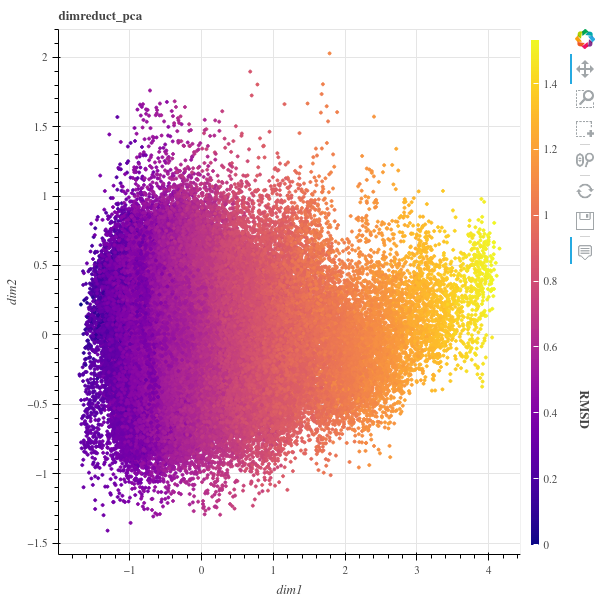
\includegraphics[width=0.5\linewidth, height=0.4\linewidth]{projects/Gustave_Li/Main_program/results/dimensionality_reduction/dimreduct_pca.png}}  
    \subfloat[kPCA\_poly]{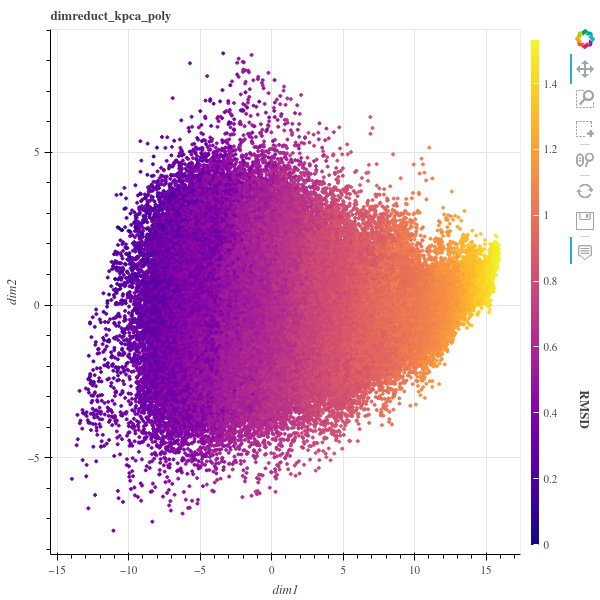
\includegraphics[width=0.5\linewidth, height=0.4\linewidth]{projects/Gustave_Li/Main_program/results/dimensionality_reduction/dimreduct_kpca_poly.png}}  \\
    \subfloat[kPCA\_rbf]{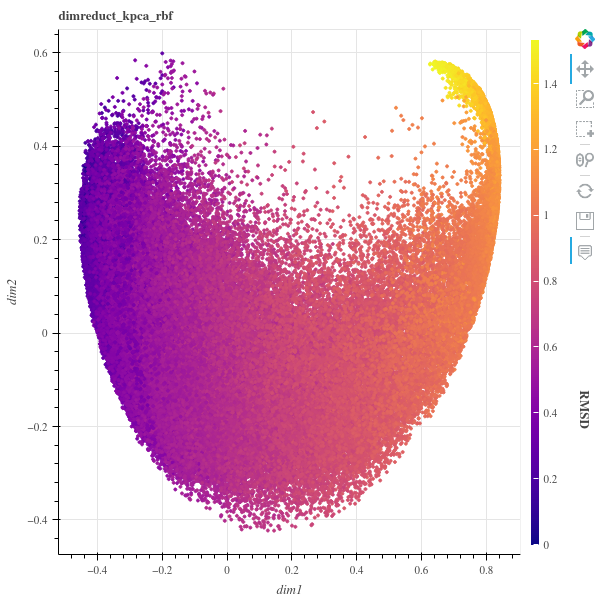
\includegraphics[width=0.5\linewidth, height=0.4\linewidth]{projects/Gustave_Li/Main_program/results/dimensionality_reduction/dimreduct_kpca_rbf.png}}  
    \subfloat[t-SNE]{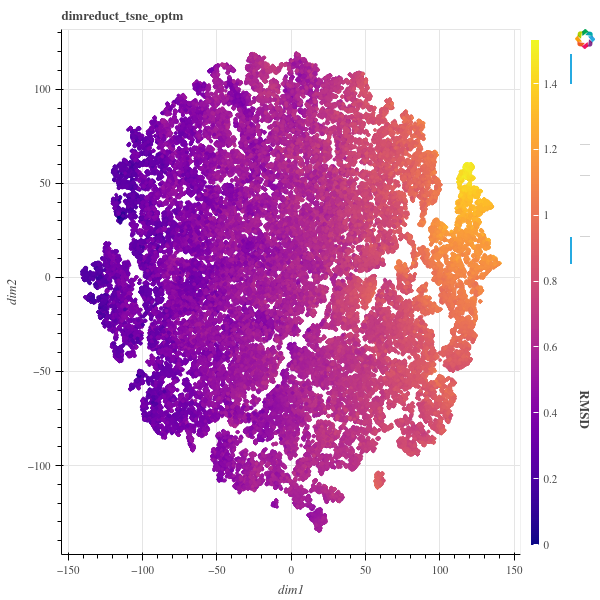
\includegraphics[width=0.5\linewidth, height=0.4\linewidth]{projects/Gustave_Li/Main_program/results/dimensionality_reduction/dimreduct_tsne_optm.png}}
    \caption{Dimensionality reduction results for descriptors. The triad indexing 87507, which lies on the far left of the graph, was chosen for the RMSD reference frame.  }
    \label{fig:dimreduct_descriptors}
\end{figure}

\subsection{Dimensionality reduction on coordinates}
\begin{figure}[H]
    \centering
    \subfloat[PCA]{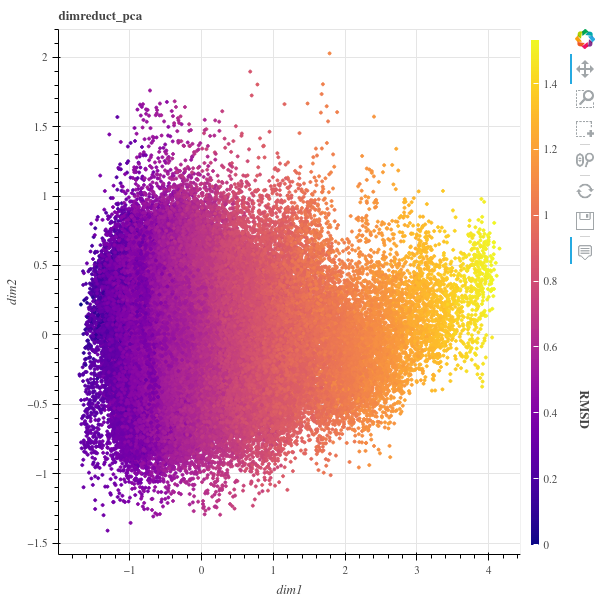
\includegraphics[width=0.5\linewidth, height=0.4\linewidth]{projects/Gustave_Li/Main_program/results/dimensionality_reduction/dimreduct_pca.png}}  
    \subfloat[kPCA\_poly]{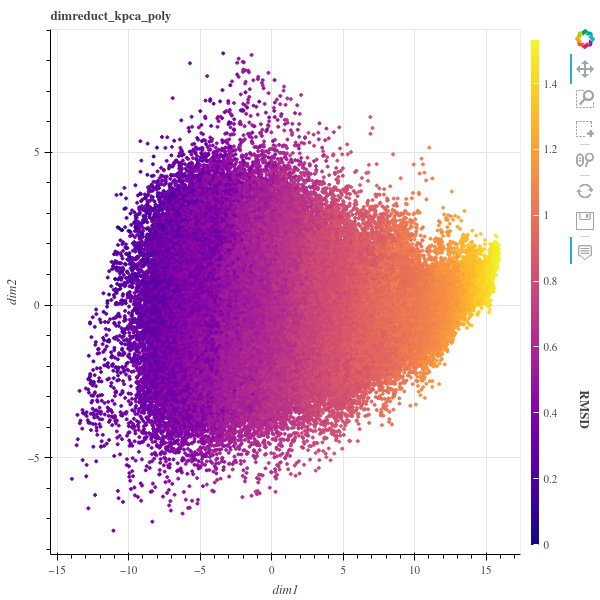
\includegraphics[width=0.5\linewidth, height=0.4\linewidth]{projects/Gustave_Li/Main_program/results/dimensionality_reduction/dimreduct_kpca_poly.png}}  \\
    \subfloat[kPCA\_rbf]{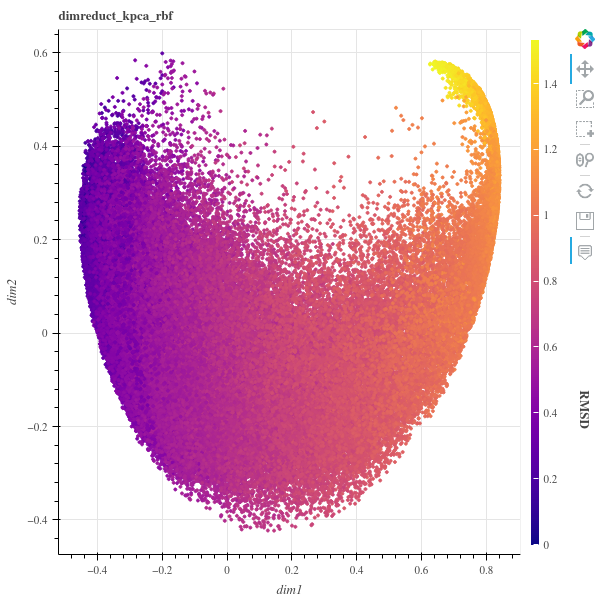
\includegraphics[width=0.5\linewidth, height=0.4\linewidth]{projects/Gustave_Li/Main_program/results/dimensionality_reduction/dimreduct_kpca_rbf.png}}  
    \subfloat[t-SNE]{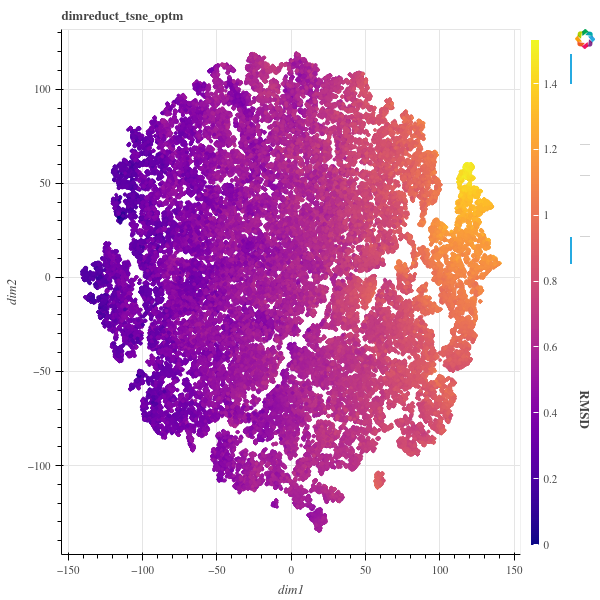
\includegraphics[width=0.5\linewidth, height=0.4\linewidth]{projects/Gustave_Li/Main_program/results/dimensionality_reduction/dimreduct_tsne_optm.png}}
    \caption{Dimensionality reduction results for descriptors. The triad indexing 87507, which lies on the far left of the graph, was chosen for the RMSD reference frame.  }
    \label{fig:dimreduct_descriptors}
\end{figure}

\pagebreak
\bibliographystyle{unsrt}
\bibliography{references.bib}

\end{document}